\section{Hướng dẫn sử dụng chương trình}
\textbf{Lưu ý:}
\begin{itemize}
    \item Cài đặt ngôn ngữ lập trình Python
    \item Cài đặt các thư viện ngoài bằng cú pháp sau trên terminal: \texttt{pip install customtkinter pillow wmi}
\end{itemize}

\textbf{Hướng dẫn chi tiết}
\begin{itemize}
    \item \textbf{Bước 1:} Tải toàn bộ thư mục mã nguồn về máy tính
    \item \textbf{Bước 2:} Vào thư mục Source, chạy file main.py bằng câu lệnh py (hoặc python) main.py trên terminal.
    \begin{figure}[H]
        \centering
        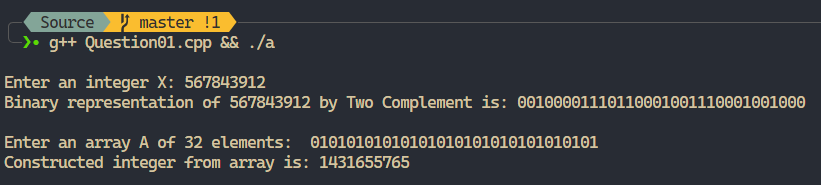
\includegraphics[width=\textwidth]{images/img1.png} 
        \caption{Giao diện khi vừa chạy chương trình.}
        \label{figure:s1}
\end{figure}
    \newpage
    \item \textbf{Bước 3:} Giao diện hiện ra, chọn phân vùng từ USB muốn đọc và bấm "Select Disk". Phần bên phải sẽ hiển thị các thông tin quan trọng của partition, phần bên trái sẽ hiển thị cây thư mục.

\begin{figure}[H]
    \centering
    \subfloat[\centering FAT32]{{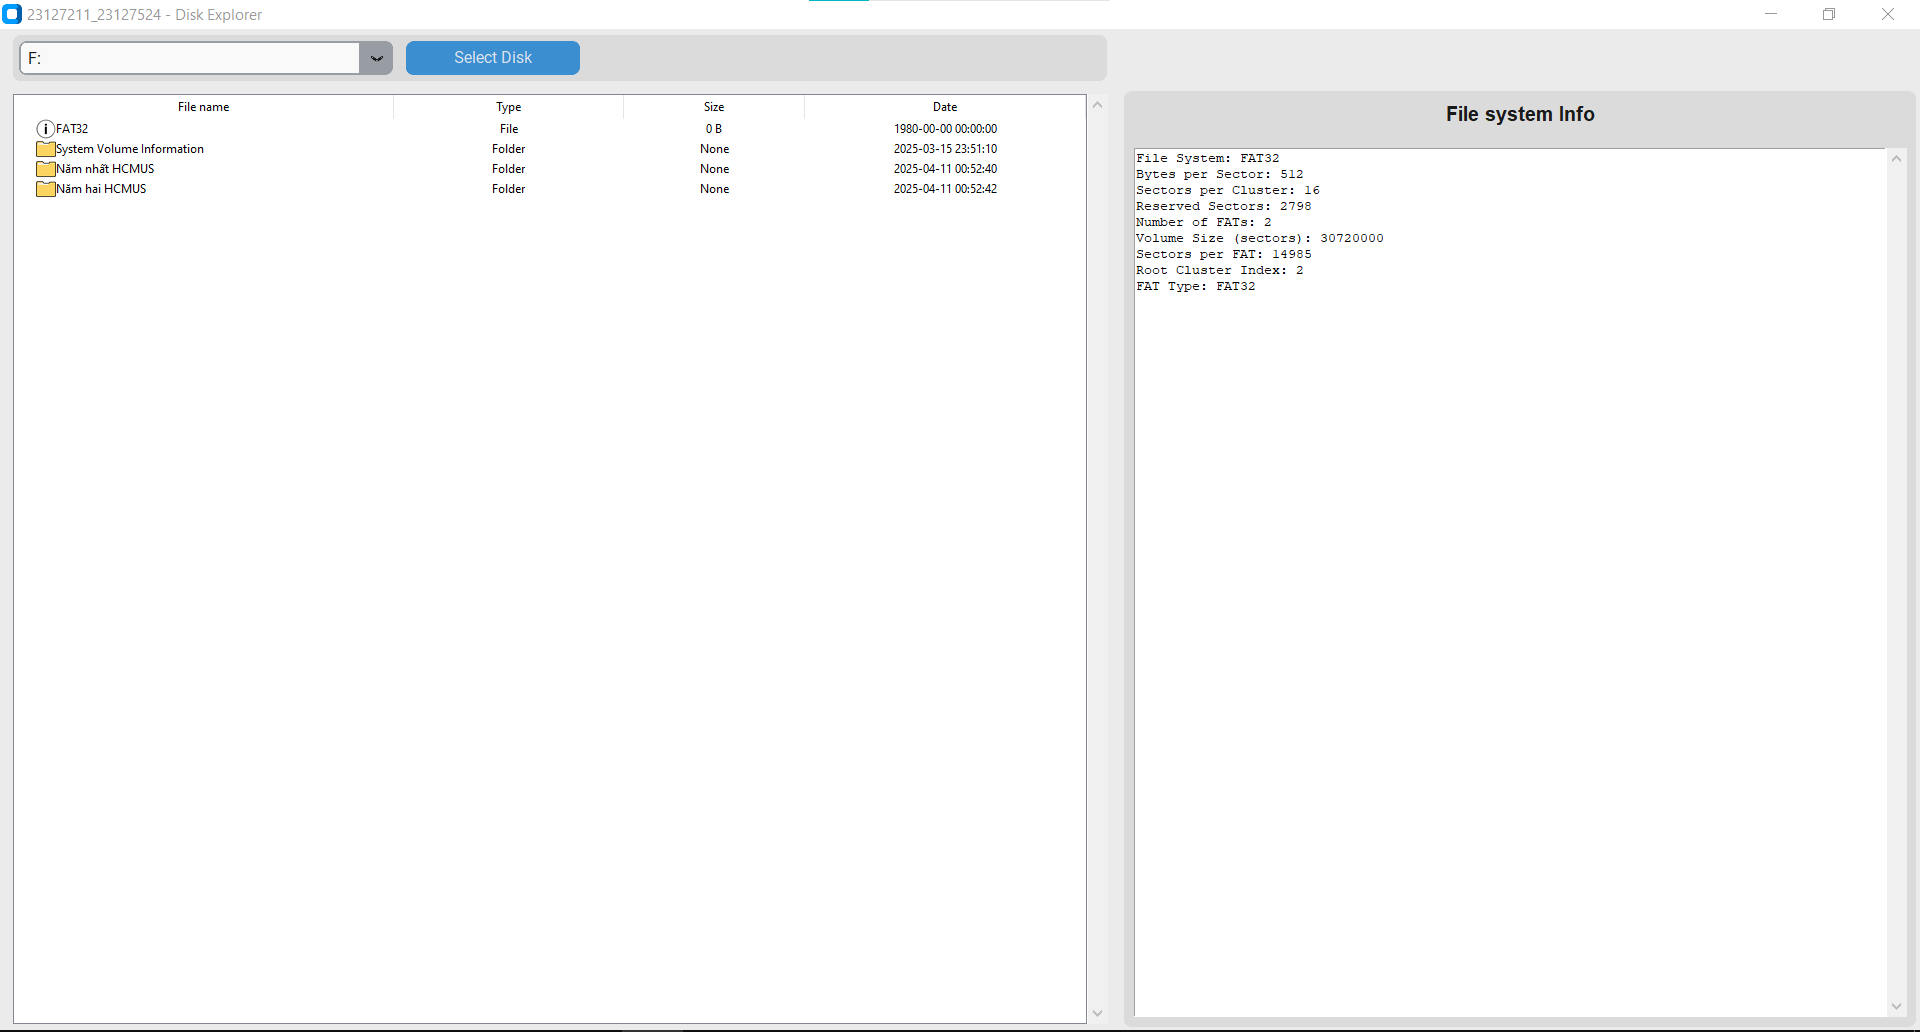
\includegraphics[width=\textwidth]{images/img2.1.png} }}%
    \qquad
    \subfloat[\centering NTFS]{{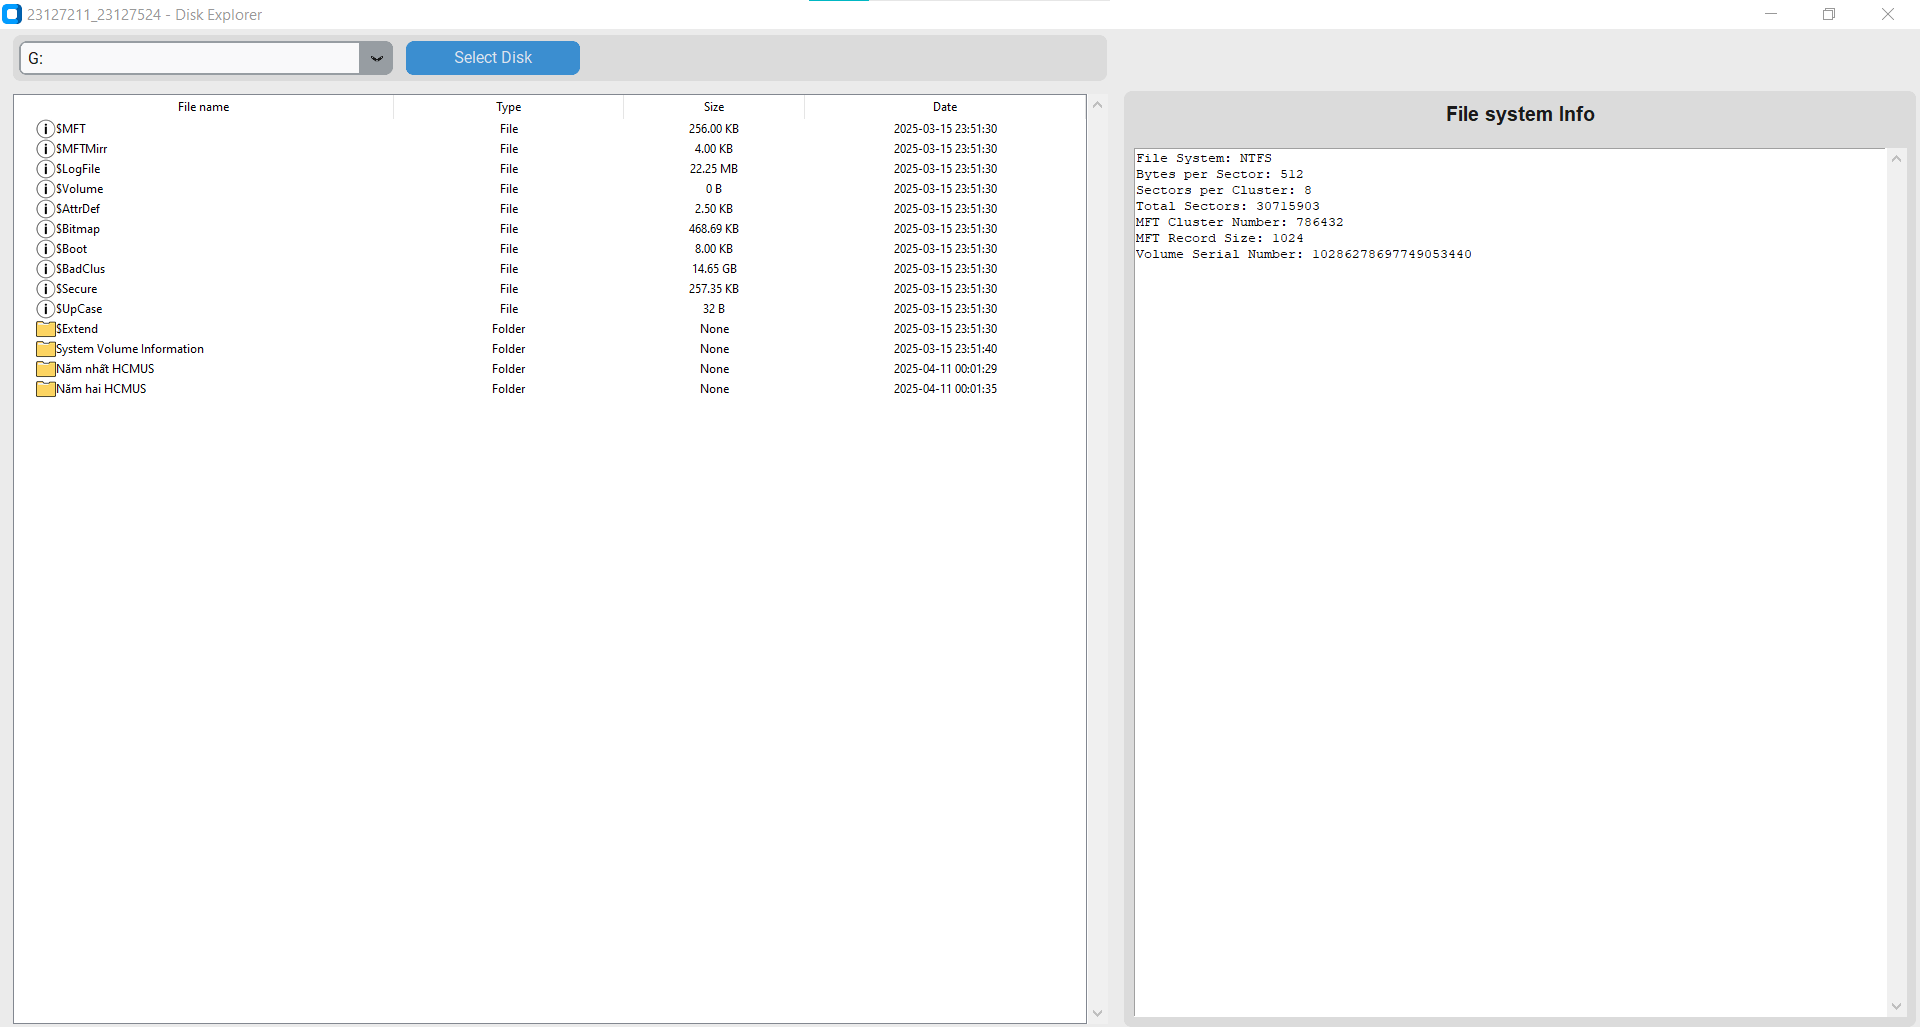
\includegraphics[width=\textwidth]{images/img2.2.png}} }%
    \caption{Giao diện chương trình sau khi chọn phân vùng}%
    \label{fig:stackArrayPush}%
\end{figure}

    \newpage
    \item \textbf{Bước 4:} Nhấp đúp chuột vào thư mục/file bạn muốn, nếu là thư mục thì điều hướng vào trong, nếu là file \texttt{.txt} thì hiển thị nội dung, nếu là định dạng file khác thì sẽ báo lỗi, nếu là item \textbf{..} thì sẽ điều hướng ra thư mục cha. 

      \begin{figure}[H]
        \centering
        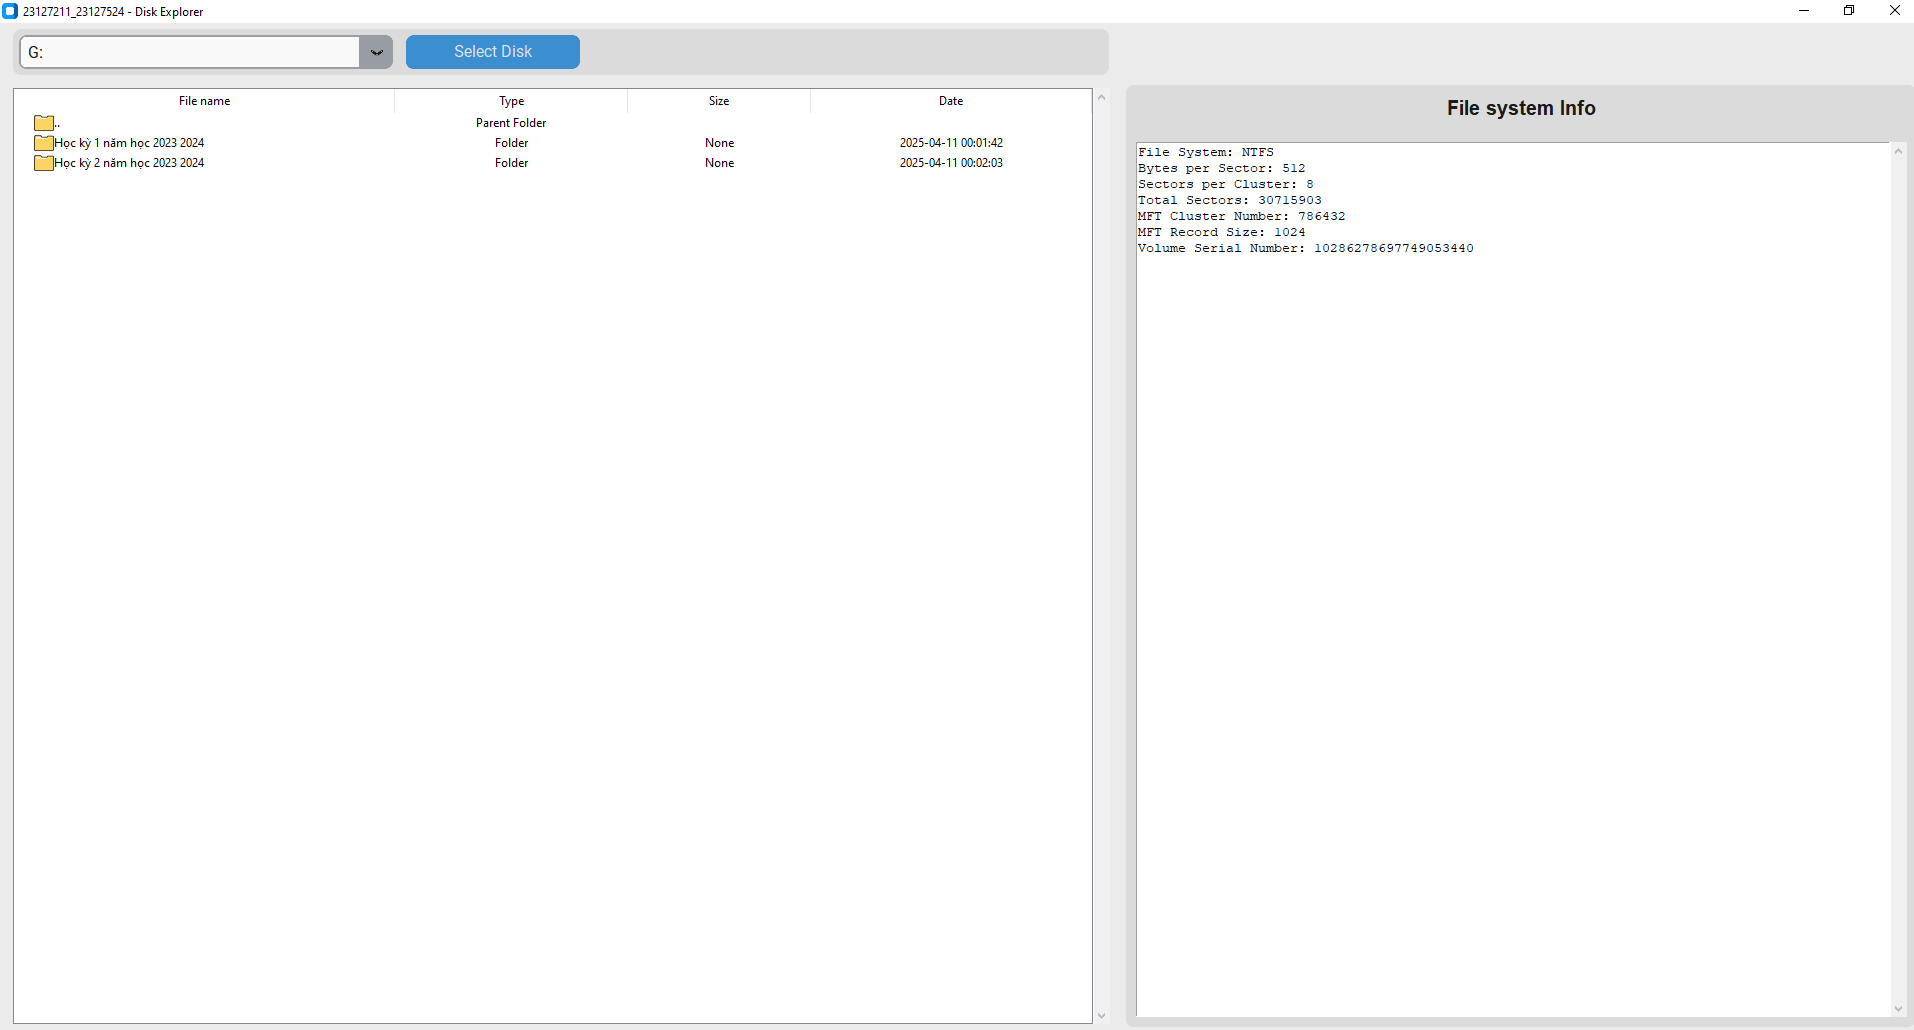
\includegraphics[width=0.8\textwidth]{images/img3.png} 
        \caption{Giao diện sau khi người dùng chọn vào thư mục.}
        \label{figure:s1}
\end{figure}

\begin{figure}[H]
        \centering
        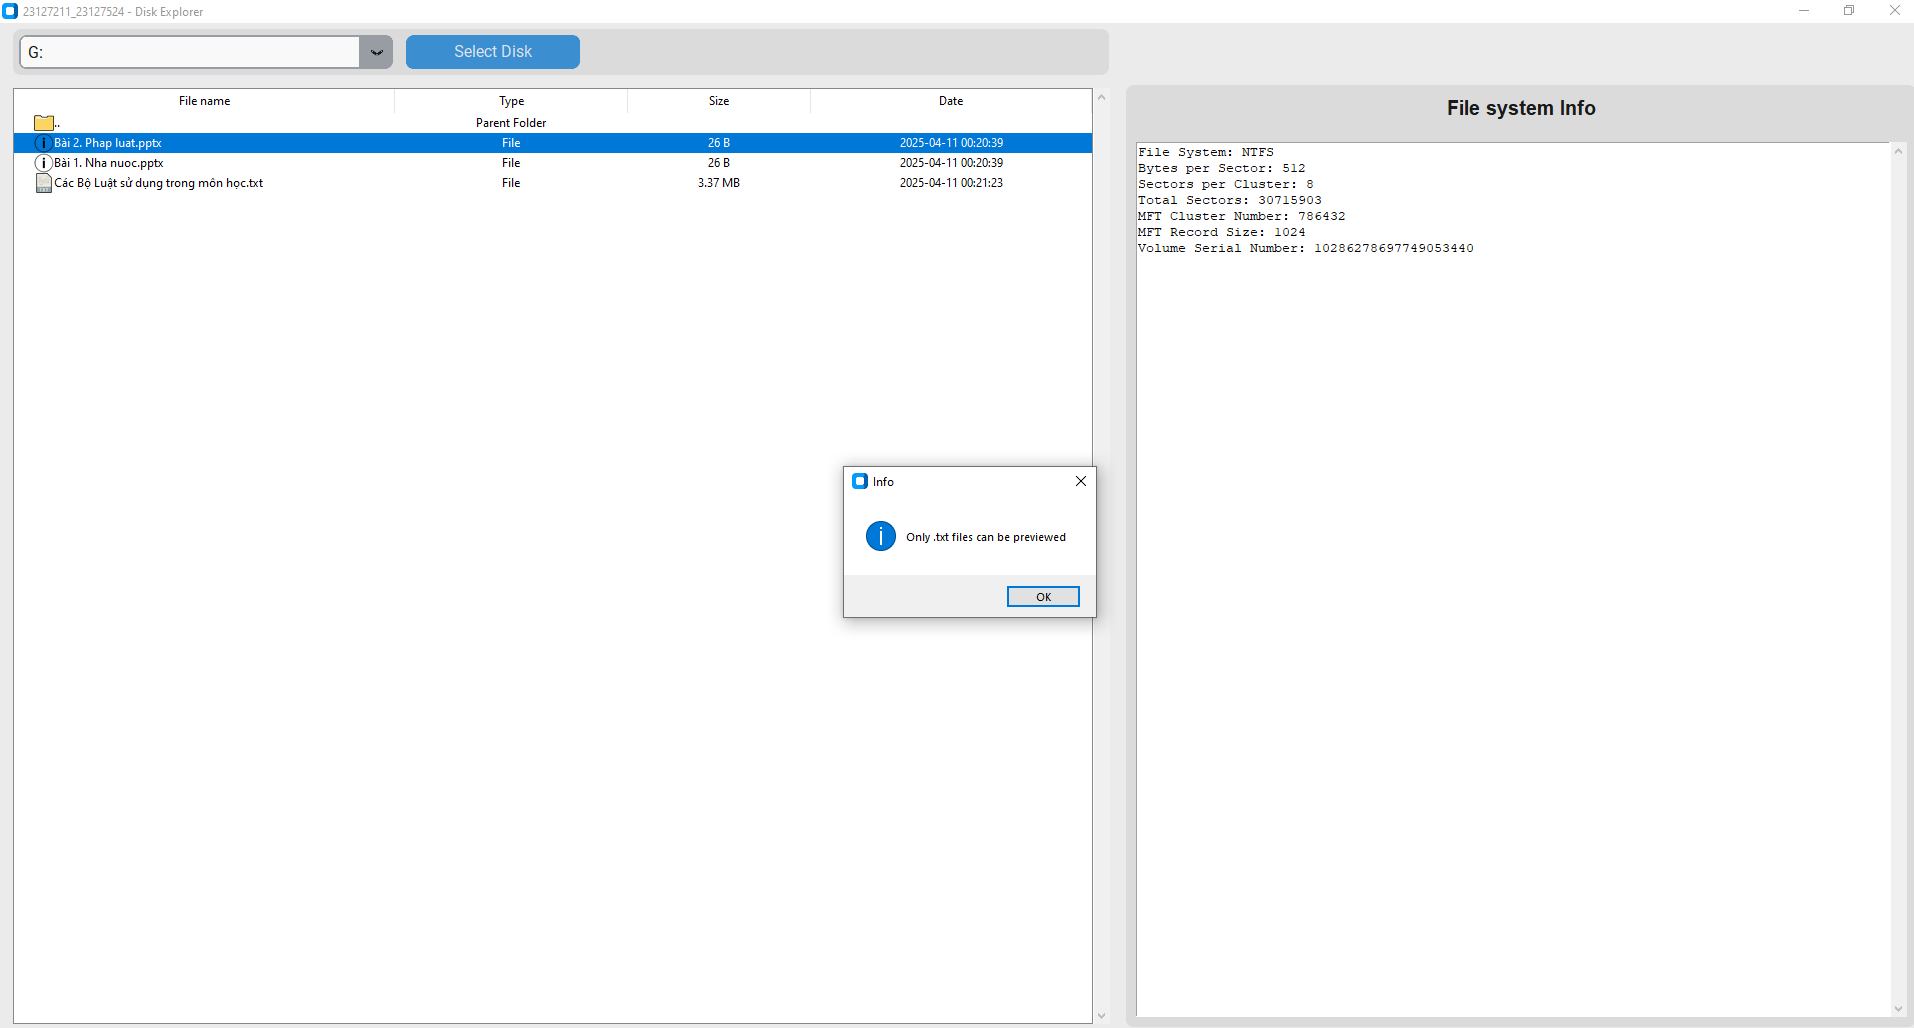
\includegraphics[width=0.8\textwidth]{images/img6.png} 
        \caption{Chương trình sẽ thông báo nếu bạn chọn file khác đuôi .txt.}
        \label{figure:s1}
\end{figure}

        \begin{figure}[H]
    \centering
    \subfloat[\centering FAT32]{{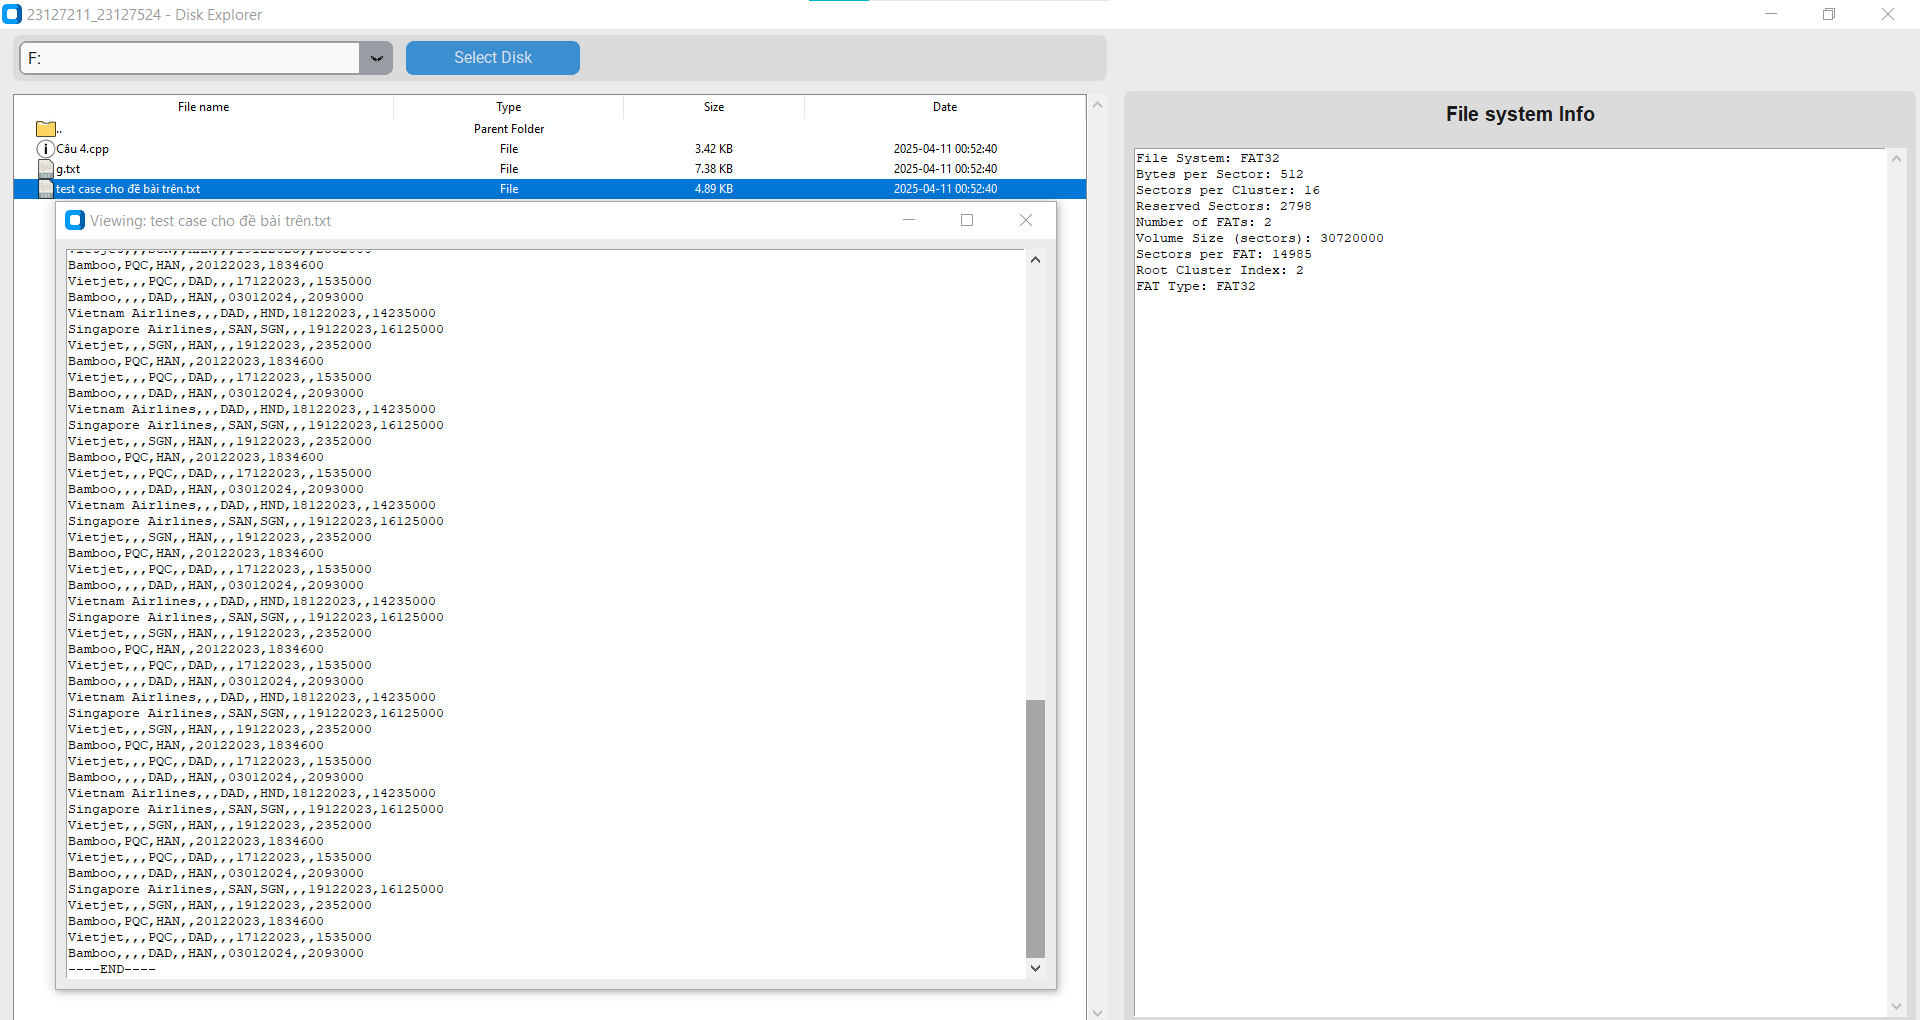
\includegraphics[width=\textwidth]{images/img4.1.png} }}%
    \qquad
    \subfloat[\centering NTFS]{{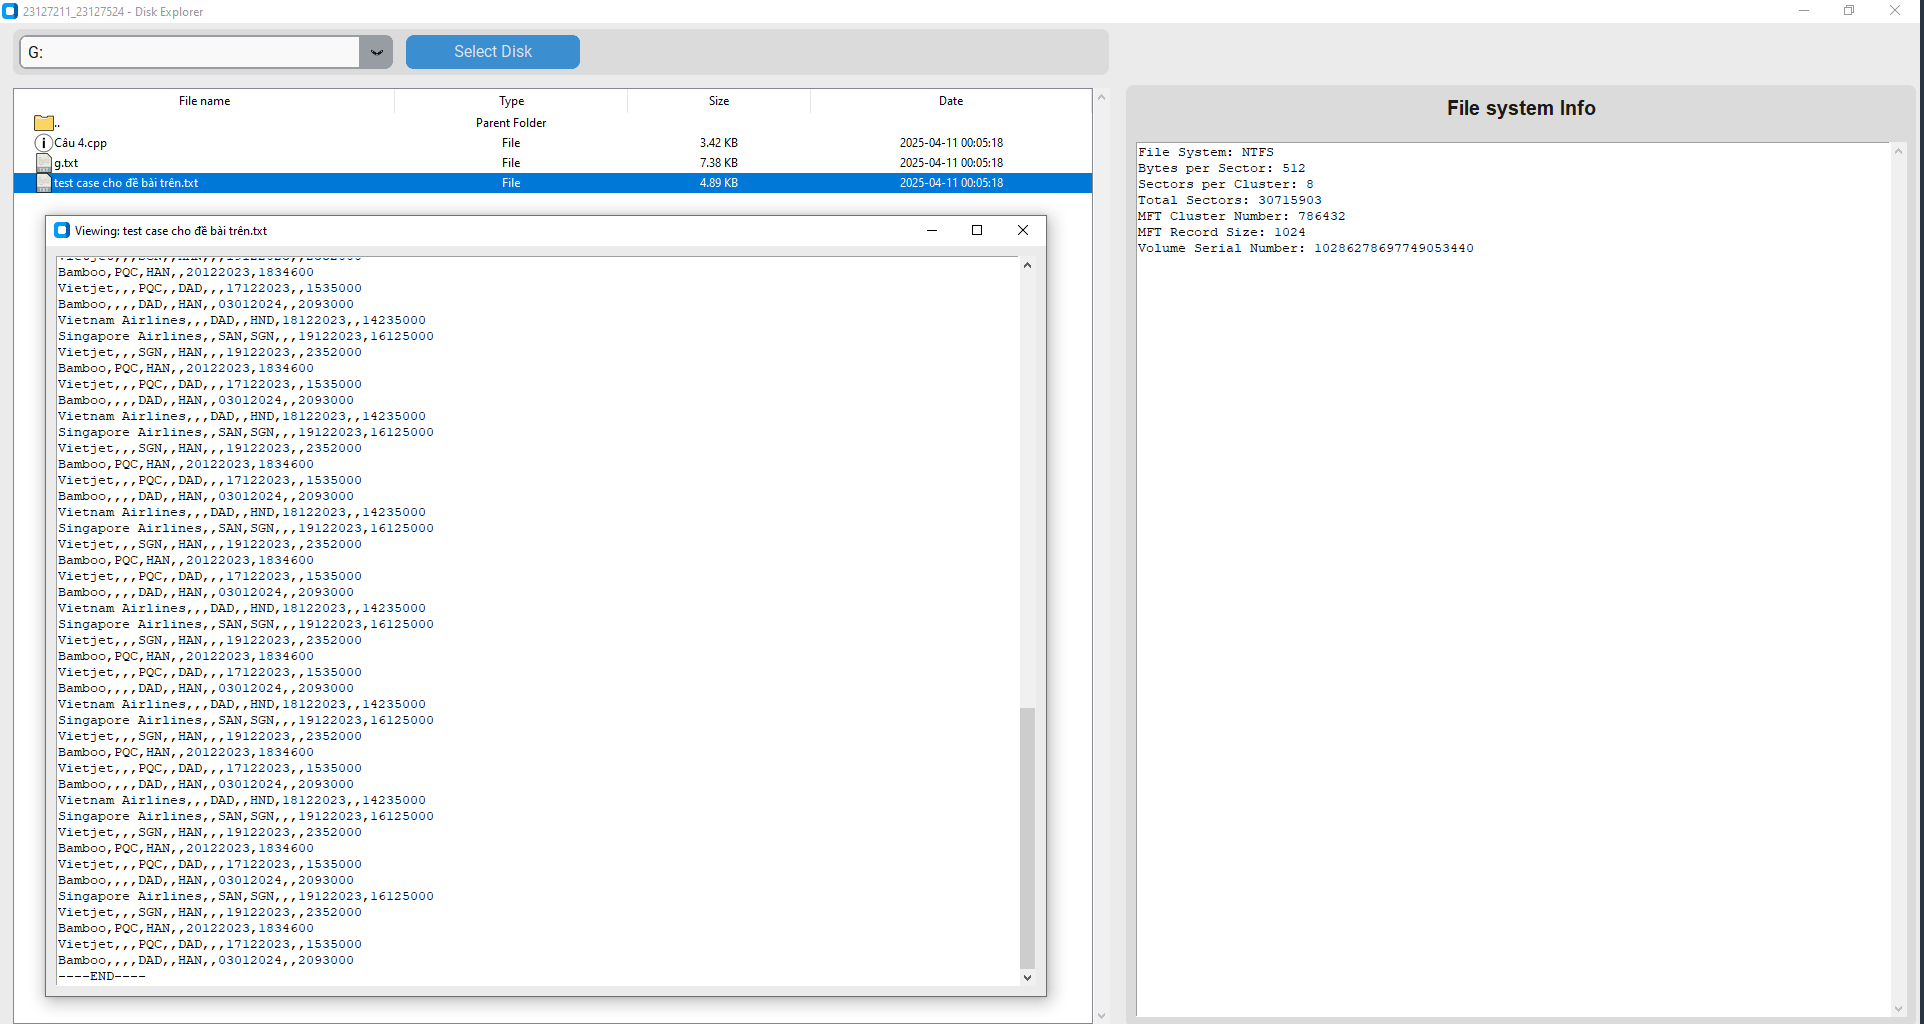
\includegraphics[width=\textwidth]{images/img4.2.png}} }%
    \caption{Giao diện đọc file đuôi .txt}
    \label{fig:stackArrayPush}%
\end{figure}

  \begin{figure}[H]
    \centering
    \subfloat[\centering FAT32]{{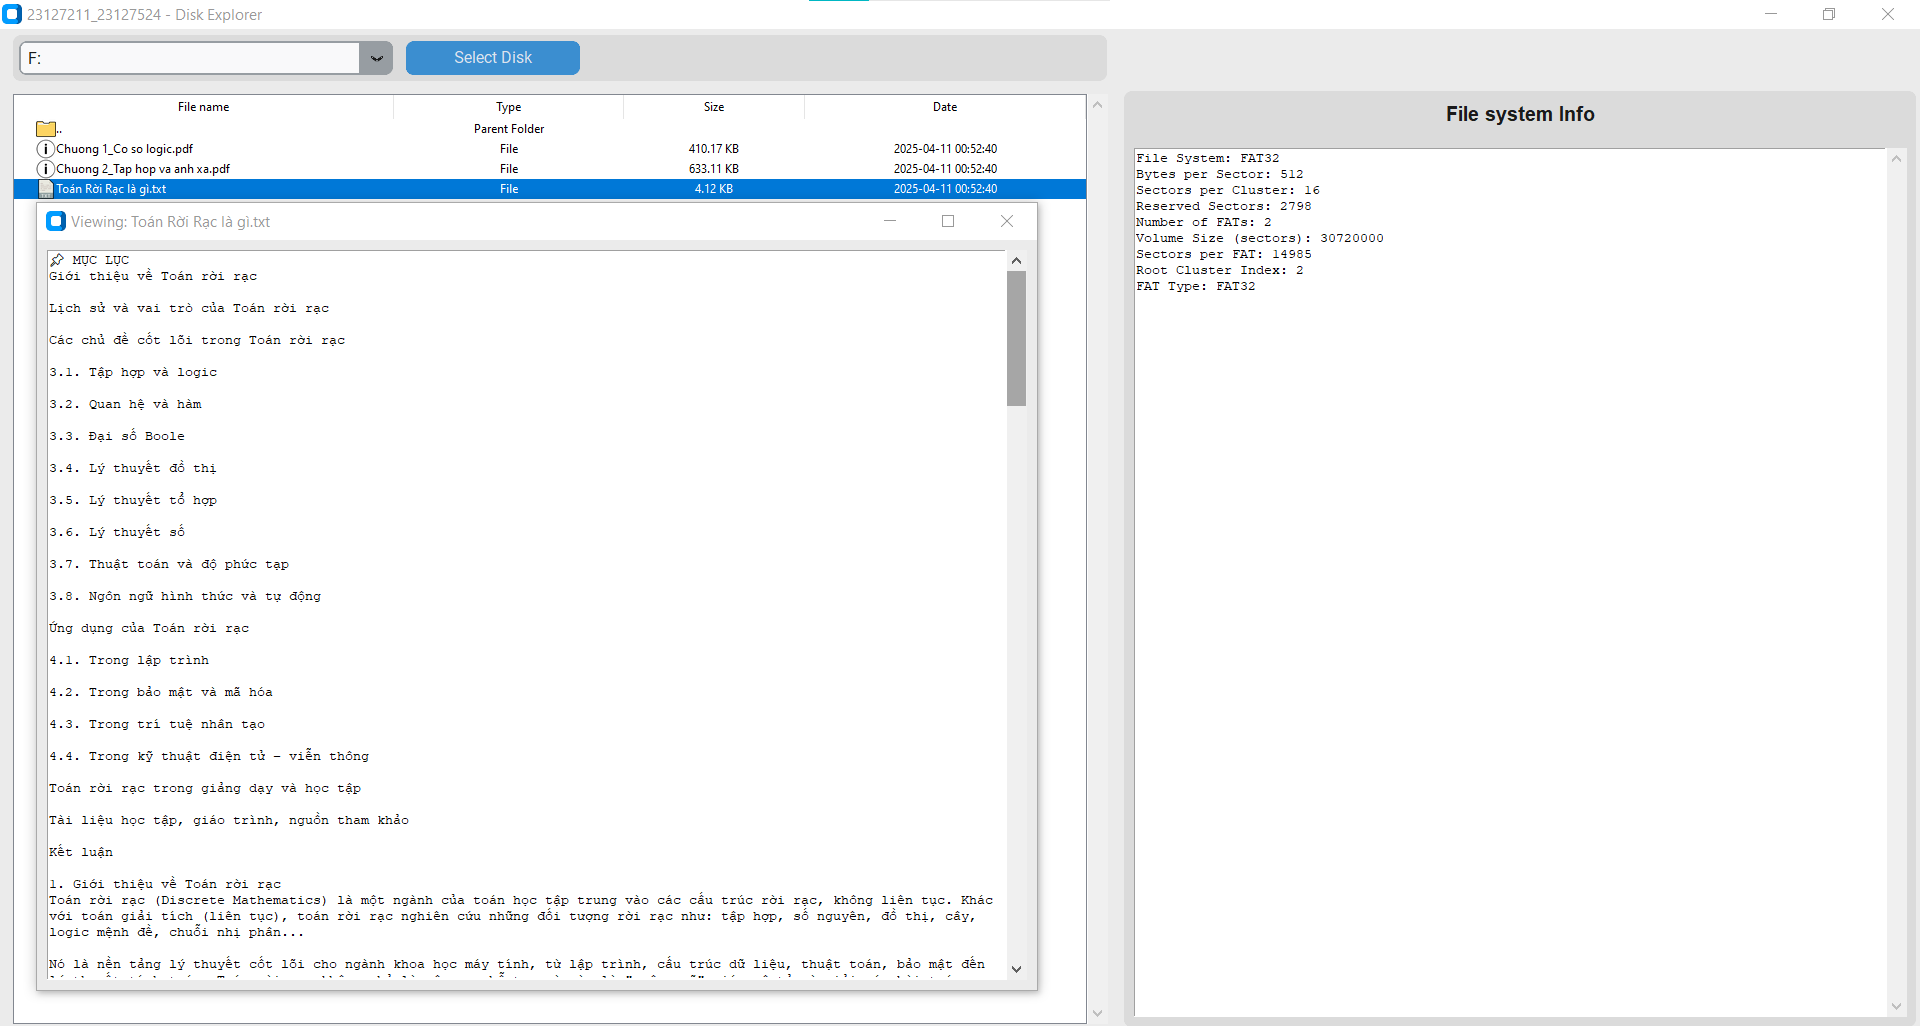
\includegraphics[width=\textwidth]{images/img5.1.png} }}%
    \qquad
    \subfloat[\centering NTFS]{{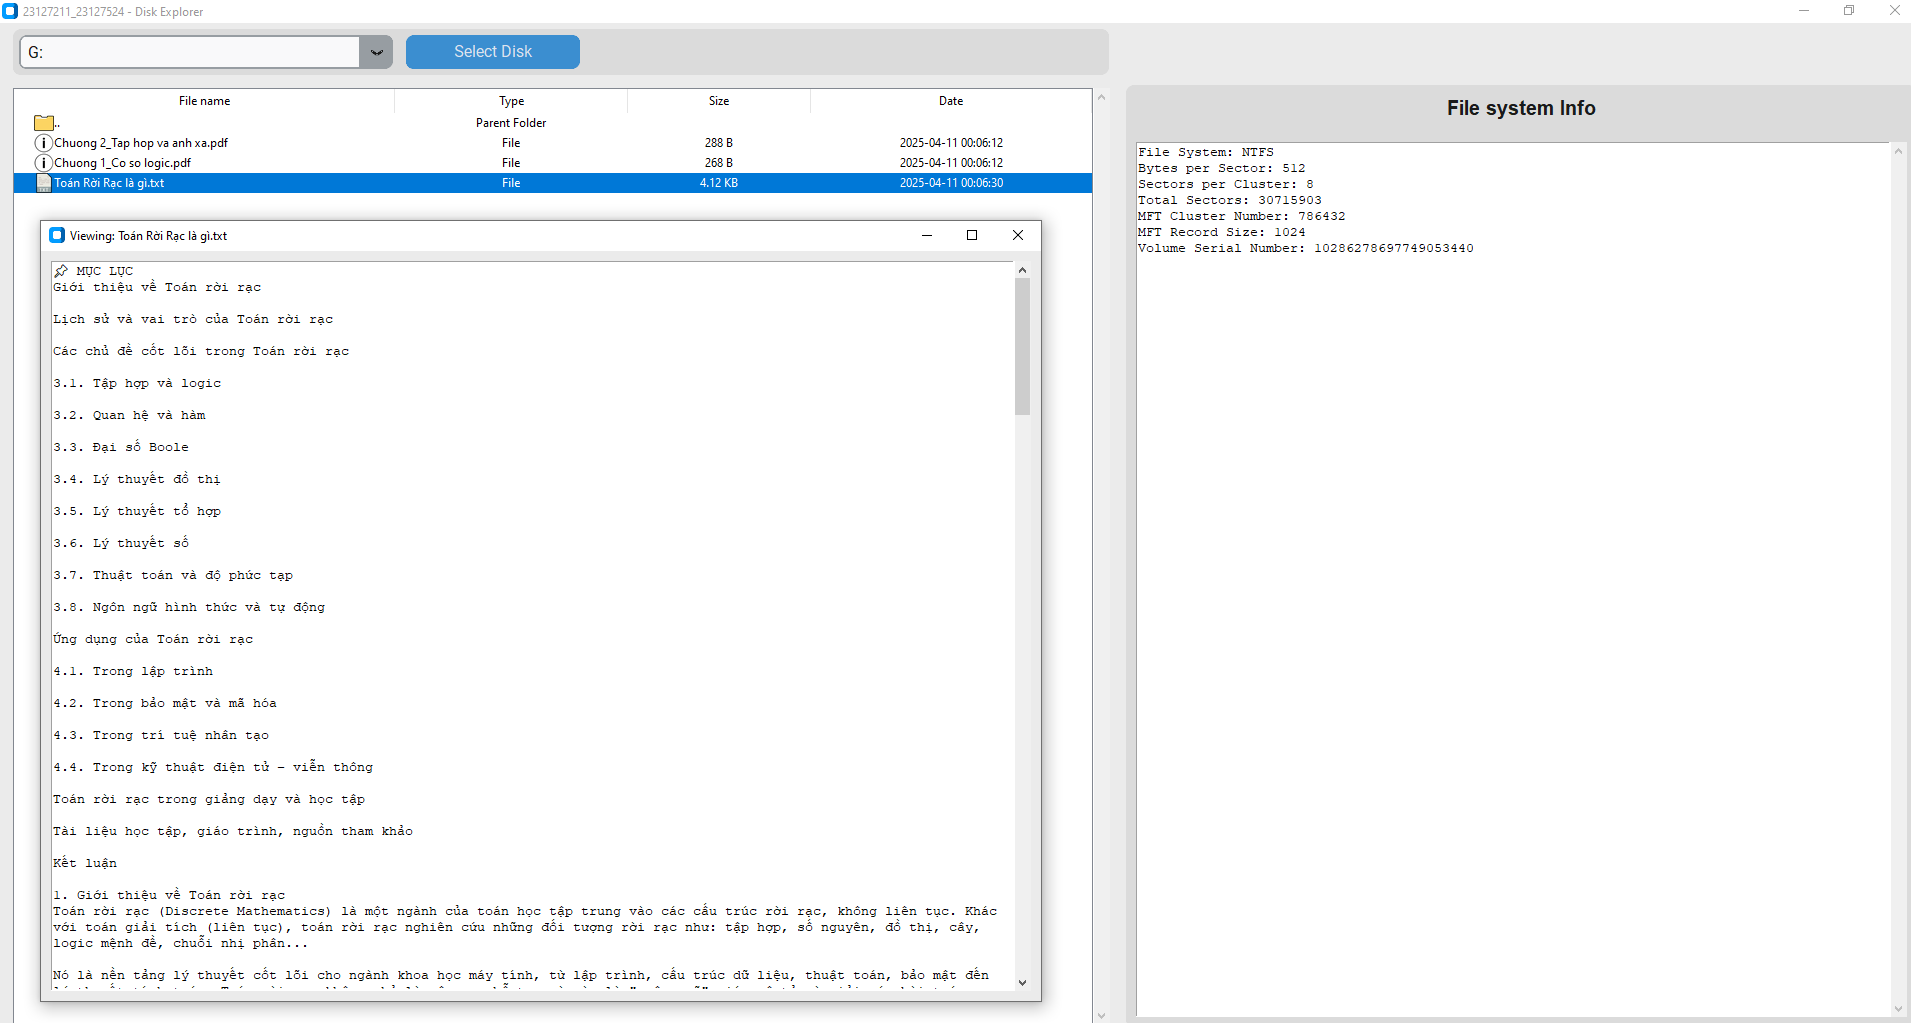
\includegraphics[width=\textwidth]{images/img5.2.png}} }%
    \caption{Đọc tốt nội dụng file kể cả file tiếng việt}
    \label{fig:stackArrayPush}%
\end{figure}


    
\end{itemize}